\documentclass[conference]{IEEEtran}
\IEEEoverridecommandlockouts
% The preceding line is only needed to identify funding in the first footnote. If that is unneeded, please comment it out.
\usepackage{cite}
\usepackage{amsmath,amssymb,amsfonts}
\usepackage{algorithmic}
\usepackage{graphicx}
\usepackage{textcomp}
\usepackage{xcolor}
\usepackage{subfig}
\usepackage{svg}
\usepackage{multirow}

\usepackage{multicol}

\usepackage[belowskip=-15pt,aboveskip=0pt]{caption}

\setlength{\intextsep}{10pt plus 2pt minus 2pt}

\usepackage{listings}

\usepackage{caption}

\usepackage{listings}

\usepackage{lipsum}
\usepackage{graphicx}
\ifCLASSOPTIONcompsoc
    \usepackage[caption=false, font=normalsize, labelfont=sf, textfont=sf]{subfig}
\else
\usepackage[caption=false, font=footnotesize]{subfig}
\fi


\usepackage{makeidx}



\lstset{
  basicstyle=\ttfamily,
}
\renewcommand*{\lstlistingname}{Code}

\definecolor{RoyalBlue}{RGB}{65,105,225}
\definecolor{Blue}{RGB}{0,0,225}
\definecolor{YellowGreen}{RGB}{154,205,50}
\definecolor{ForestGreen}{RGB}{34,139,34}


\lstset{ 
  linewidth=8.5cm,
  language=R,                     % the language of the code
  basicstyle=\scriptsize\ttfamily, % the size of the fonts that are used for the code
  numbers=left,                   % where to put the line-numbers
  numberstyle=\scriptsize\color{Blue},  % the style that is used for the line-numbers
  stepnumber=1,                   % the step between two line-numbers. If it is 1, each line
                                  % will be numbered
  numbersep=5pt,                  % how far the line-numbers are from the code
  backgroundcolor=\color{white},  % choose the background color. You must add \usepackage{color}
  showspaces=false,               % show spaces adding particular underscores
  showstringspaces=false,         % underline spaces within strings
  showtabs=false,                 % show tabs within strings adding particular underscores
  frame=single,                   % adds a frame around the code
  rulecolor=\color{black},        % if not set, the frame-color may be changed on line-breaks within not-black text (e.g. commens (green here))
  tabsize=2,                      % sets default tabsize to 2 spaces
  captionpos=b,                   % sets the caption-position to bottom
  breaklines=true,                % sets automatic line breaking
  breakatwhitespace=false,        % sets if automatic breaks should only happen at whitespace
  keywordstyle=\color{RoyalBlue},      % keyword style
  commentstyle=\color{YellowGreen},   % comment style
  stringstyle=\color{ForestGreen}      % string literal style
} 

\usepackage{amssymb}% 
\usepackage{pifont}% 
\newcommand{\cmark}{\ding{51}}%
\newcommand{\xmark}{\ding{55}}%


\def\BibTeX{{\rm B\kern-.05em{\sc i\kern-.025em b}\kern-.08em
    T\kern-.1667em\lower.7ex\hbox{E}\kern-.125emX}}
\begin{document}

\title{Performance of Windows vs Linux approach for image rendering}

\author{
\IEEEauthorblockN{Allan Sánchez Masís}
\IEEEauthorblockA{\textit{Computer Science School} \\
\textit{Instituto Tecnológico de Costa Rica}\\
allansanchezmasis@gmail.com}

}

\maketitle

\begin{abstract}
This paper shows a comparison through image rendering time, of different Operating System implementations; Compiled to run natively on Windows, in a Ubuntu virtual machine and Debian virtual machine with Windows as a host, and compiled for Ubuntu, running on Windows Linux Subsystem. The comparison is to evaluate the performance of Linux, Windows, virtual machine and Windows Linux subsystem, via statistical analysis.  It was determined that there is no significant statistical difference to say that Ubuntu is better than Windows, even Ubuntu, Windows and Ubuntu in a virtual machine are similar but better than Debian in a virtual machine and than WSL.

\end{abstract}

\begin{IEEEkeywords}
Linux, Windows, Ubuntu, Debian, ANOVA
\end{IEEEkeywords}

\section{Introduction}
Understanding the Operating System (OS) is crucial in computer sciences because the OS is what makes the
hardware work with the software like an
interface that allows the executions of processes \cite{dhamija2012demographics}. Thus, it is necessary to understand which OS gives the best performance and facilities according with the different user tasks, it is critical to focus more the researches not only in their qualities, also with numbers and metrics to quantify their performance. \par
There are different well-known features which OS like Windows and Linux offer for the different spectrum of users and their needs. There are very well-known features of this OS, for example, Linux is free to obtain, meanwhile, Microsoft products are available for a considerable fare \cite{dhamija2012demographics}, and the licenses has a price for every machine where are installed  \cite{duran2006analisis}, on the other hand, Windows is more popular than Windows \cite{duran2006analisis}, thus, typical users prefers Windows because it is what they probably will need for their office jobs, studies, games, and so on, therefore, people is not much familiar with Linux as Windows and require more expertise and learning curve \cite{dhamija2012demographics}.\par
Considering technical aspects, vast of Linux programs are Open Source, thus, users are able to modify the feature of different software packages according to their necessities, nevertheless, Linux can only run binaries that have been  created for it, whereas Windows has a lot of of programs, significantly more than any other OS \cite{dhamija2012demographics}.\par

This paper shows a comparison using image rendering time, of different Operating System implementations; Compiled to run on Windows and Ubuntu both natively, running on virtual machines with Ububtu and Debian both with Windows as a host, and compiled for Ubuntu, running on Windows Linux Subsystem. To make the comparison is used statistical analysis (Anova). The scenes used for rendering are depicted in \ref{fig_scenes}. Thus, with the proposed study it possible to identify, If Windows is slower than Linux, by how much is it? How can a valid comparison be made between
both operating systems? Which is better? Run an application compiled for
run on Windows natively, or run it on a
Linux virtual machine on Windows? How is the performance of the Windows Subsystem for 
Linux in this scenario? Is it better to run it in WSL,
which natively for Windows?


\begin{figure}[t]
    \centering
   % \subfloat[subc\label{1a}]{
  \subfloat[\label{1a}]{%
       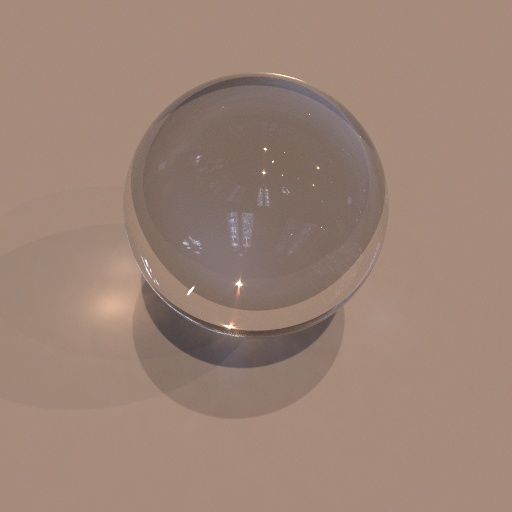
\includegraphics[width=0.45\linewidth]{figures/caustic-proj (1).jpg}}
    \hfill
  \subfloat[\label{1b}]{%
        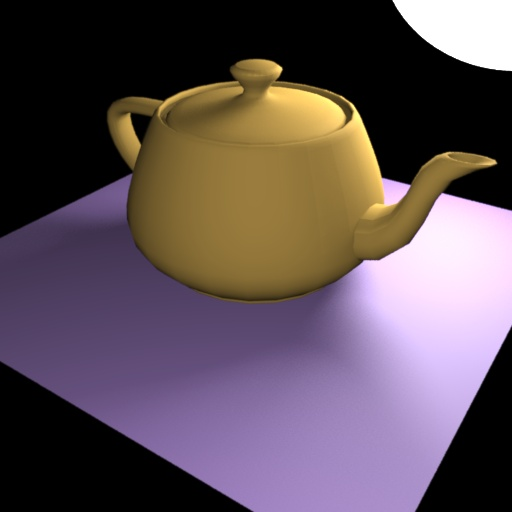
\includegraphics[width=0.45\linewidth]{figures/teapot-area-light.jpg}}
    \\
  \subfloat[\label{1c}]{%
        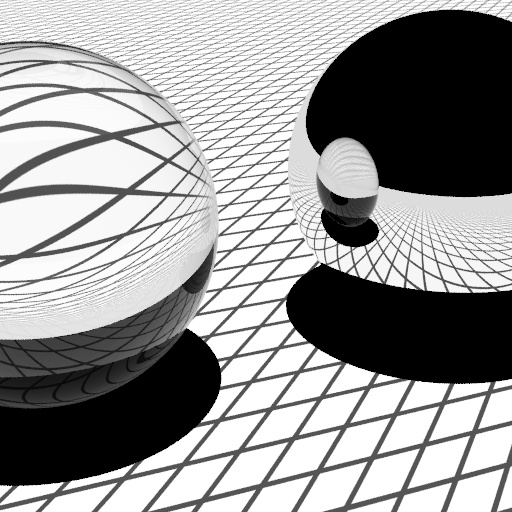
\includegraphics[width=0.45\linewidth]{figures/spheres-differentials-texfilt.jpg}}
    \hfill
  \subfloat[\label{1d}]{%
        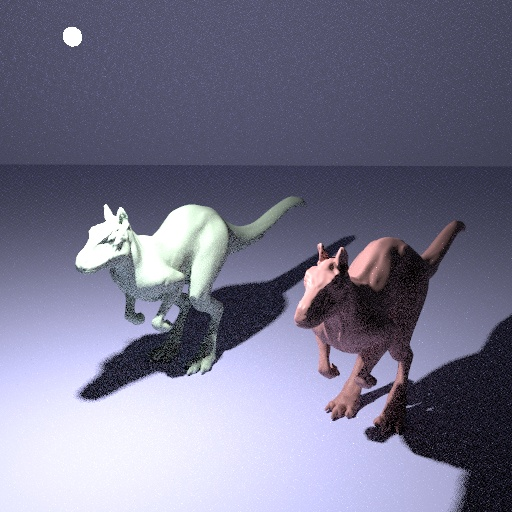
\includegraphics[width=0.45\linewidth]{figures/killeroo-simple.jpg}}
  \caption{Chosen Scenes used to validate performance with PBRT-V3. (a) scene 1 , caustic-proj \cite{PBRTdata}, (b) scene 2, teapot-area-light \cite{PBRTdata}, (c) scene 3, spheres-differentials-texfilt \cite{PBRTdata}, and (d) scene 4, killeroo-simple \cite{PBRT}.}
  \label{fig_scenes} 
\end{figure}



\subsection{Theoretical Background}
Image rendering is important in video industries like movies, animation, 3D video games, an so on because, rendering is the process of creating an image from a 3D scene description. PBR try to imitate reality by modeling the interplay of light and matter using real physics concepts \cite{PBR}. \par
The accelerator is one of the studied factors in this research, as was mentioned, two possibilities are analyzed, the kd-tree and BVH, kd-tree is a variation of Binary space partitioning (BSP) trees, which subdivide space with planes, however, kd-tree  restricts the divided plane to be perpendicular to one of the coordinate axes; which makes  creation of the tree more efficient. Meanwhile, BVH is a  ray intersection acceleration method based on primitive subdivision, which are partitioned into a hierarchy of separate sets  \cite{PBR}.\par
PBR involves vector and infinitesimal calculus of complex real-physics equations, therefore, it really takes advantage of the software and hardware resources to carry out the rendering, so it is a good option to evaluate the performance of the OS in their different scenarios.
\subsection{Related Work}
There are different studies which involve Linux and Windows comparisons,  \cite{duran2006analisis} analyzed web programming tools (PHP, ASP and JSP) using the Operative System Linux and Windows, they studied variables like Answer time, complexity, data base integrity and other. However, their focus is not the OS performance, and even so, they said that it cannot be stated definitively that one tool is better than the other; what was verified is that each one has
strengths and weaknesses based on the circumstances, this is an evidence of the necessity to study more the OS impact in the performance for the different tasks.\par 
In \cite{dhamija2012demographics}, a qualitative comparison is done between Linux and Linux, and quantitative comparison is scarcity, and the comparison is more skewed in favor of Linux, without sufficient numerical support. This further reaffirms the need for quantitative studies that compare the different scenarios and that these results are statistically supported.\par
This paper presents a comparison of different OS, the evaluation is done measuring the rendering time of (PBR \cite{PBR}) program, specifically the third version (PBRT-v3) \cite{PBRT}, the scenarios are five: Compiled to run natively on Windows, also natively on Ubuntu, in an Ubuntu virtual machine (U-VM) and a Debian virtual machine (D-VM) using Windows as the host, as well as compiled for Ubuntu operating on the Windows Linux Subsystem (U-WLS). This scenarios under test are studied with 3 factors, the accelerator (kd-tree and BVH), the resolution ($256 \times 256$ and $512 \times 512$), and 4 scenes depicted in Fig.\ref{fig_scenes}. To make the comparison it is used statistical analysis based on Anova. 

\section{Design Proposal}
Table \ref{tab_var} depicts the factors, and the levels to make the experiments and the statistical analysis. To make a statically correct comparison,  Multivariate Multi-Factor ANOVA (for short ANOVA) and pairwise t-test are used. Using all the factors in the table, 80 possible combinations can be made, so the same number of repetitions will be taken to make a fair comparison in the ANOVA and the pairwise t-test. The number of repetitions chosen is two, since it is the minimum necessary for there to be a variance to calculate and due to time limitations, since there are scenes that take more than an hour to render, therefore, the total number of samples is 160.
\begin{table}[t]
\centering
\caption{Experiment Factors.}
\begin{tabular}{cccc}
\hline
\textbf{\begin{tabular}[c]{@{}c@{}}OS \\ Approach\end{tabular}}                & \textbf{Scene}                                        & \textbf{Accelerator}                                  & \textbf{Resolution}                                                         \\ \hline
\begin{tabular}[c]{@{}c@{}}Windows\\ Ubuntu\\ U-VM\\ D-VM\\ U-WSL\end{tabular} & \begin{tabular}[c]{@{}c@{}}1\\ 2\\ 3\\ 4\end{tabular} & \begin{tabular}[c]{@{}c@{}}Kd-tree\\ BVH\end{tabular} & \begin{tabular}[c]{@{}c@{}}$512 \times 512$\\ $256 \times 256$\end{tabular} \\ \hline
\end{tabular}
\label{tab_var}
\end{table}
ANOVA assumptions are validated and data transformation is done when this assumption are not achieved, it is tested from the least aggressive transformation (square root), followed by the cube root and the natural logarithm.\par
Data is collected in a way that the computer is almost only running PBRT-V3, to avoid the intervention of another factors, and also, trying to follow the same conditions of Operating Systems, for example, Ubuntu natively, on VM, and with WSL were installed the same version, this aspects of the Design of Experiment (DoE) are explained in methodology.

\subsection{Methodology}
Multi-Factor ANOVA is used to analyzed statistically the behaviour of all possible combinations of all the scenarios, thus, there is not missed information or skews to a specific factor or level of the factors. And, pairwise t-test to make the port-hoc validation since type I error is reduced.\par
For all the scenarios, it is used the same computer with 4 cores (2.7GHz), 8GB of RAM. The version of windows 10 home was used, and the same hard drive was partitioned with ubuntu, for the scenario where both run natively. The scenarios that required Ubuntu all ran on the same Ubuntu 20.04 LTS release. And the version of Debian is 11.3.0. All statistical analysis is done in R. \par
For Ubuntu and Debian in Virtual machine, the same setup was used of the virtual machine, 4GB of RAM and 2 core, due to it is not recommended use all the resources. \par
When PBRT-V3 was executed to take the data, it was tried not to run other unnecessary programs, all the data was taken in a log, seconds from the date command to record it.\par



\section{Results and Discussion}
Fig. \ref{fig_summary} depicts the summary of data; there is a 160 samples as expected, the scene that lasted the longest is 4936.7 seconds (1 hour 22 minutes) and the shortest one is 2 seconds. This gives an intuition that data is not homoscedastic, and it is necessary to validate it with the ANOVA assumptions.
\begin{figure}[b]
    \centering
    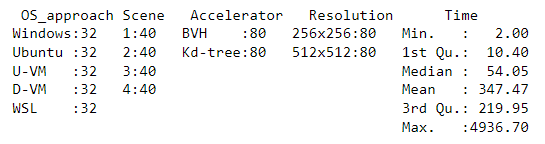
\includegraphics[scale=0.6]{figures/summary.png}
    \caption{Summary of data.}
    \label{fig_summary}
\end{figure}

Fig.\ref{fig_assumptions} demonstrate the expected, without data transformation residuals are not normal and data is not homoscedastic, cube root transformation was the one with a better visual fit of transformation, thus, this is the chosen one to make ANOVA and pairwise t-test.

\begin{figure}[h]
    \centering
   % \subfloat[subc\label{1a}]{
  \subfloat[\label{1a}]{%
       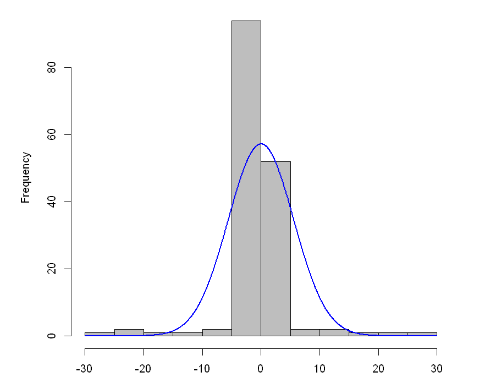
\includegraphics[width=0.45\linewidth]{figures/hist1.PNG}}
    \hfill
  \subfloat[\label{1b}]{%
        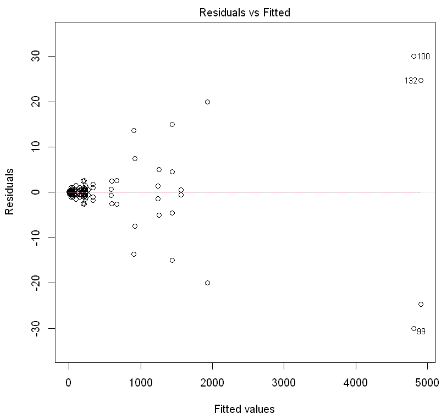
\includegraphics[width=0.45\linewidth]{figures/homo1.png}}
    \\
  \subfloat[\label{1c}]{%
        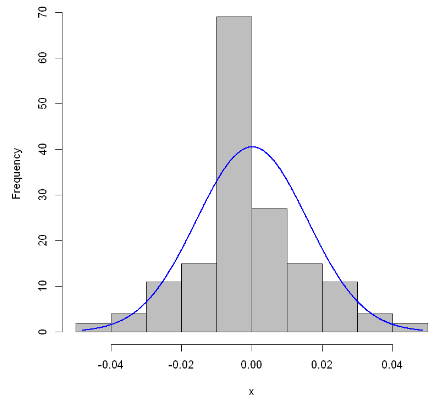
\includegraphics[width=0.45\linewidth]{figures/hist2.PNG}}
    \hfill
  \subfloat[\label{1d}]{%
        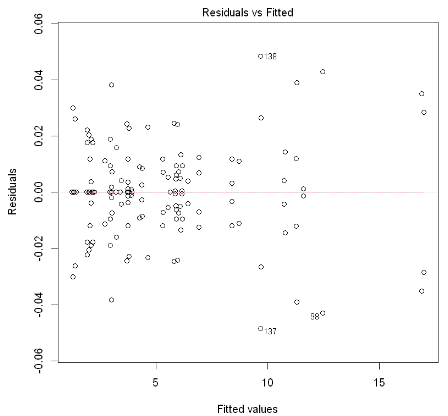
\includegraphics[width=0.45\linewidth]{figures/homo2.PNG}}
  \caption{Anova assumptions (a) no transformation bar chart, (b) no transformation variance plot, (c) Data transformation cube root bar chart, and (d) (c) Data transformation cube root variance plot.}
  \label{fig_assumptions} 
\end{figure}

The ANOVA result for transformed data is shown in Fig.\ref{fig_anova}, and it is possible to see that all the factors an their interactions affects the performance due to p-value<0.05, thus, it possible to plot the time-transformed mean-whisker and compute the respective pairwise t-test.


\begin{figure}[tb]
    \centering
    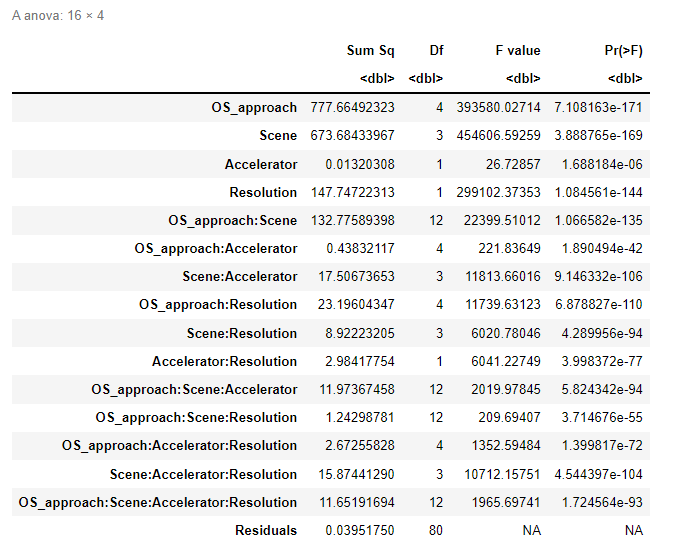
\includegraphics[scale=0.5]{figures/anova.png}
    \caption{ANOVA for transformed data.}
    \label{fig_anova}
\end{figure}

The time-transformed mean-whisker plot considering only the OS approach is shown in Fig.\ref{fig_mean_1}; it seems that Ubuntu is better than any approach, followed by windows and that the worst of all is WSL together with Debian, and that using an Ubuntu virtual machine is just as good as Windows, however, we cannot be sure until we verify that they are statistically different with the pairwise t-test.

\begin{figure}[ht]
    \centering
    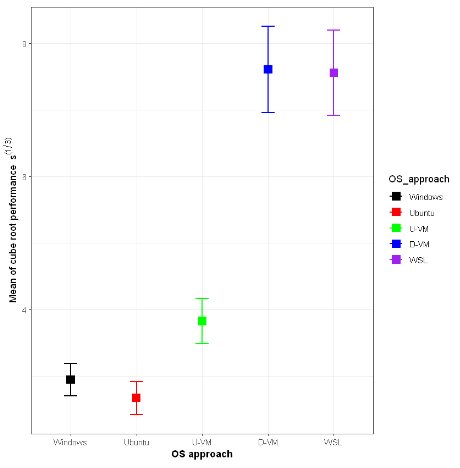
\includegraphics[scale=0.5]{figures/mean1.PNG}
    \caption{Time-transformed mean-whisker plot as a function of the OS approach.}
    \label{fig_mean_1}
\end{figure}


Fig. \ref{fig_ttest_1} shows that in reality Ubuntu, Windows and Ubuntu in a virtual machine are statistically similar, there is not enough difference to say that Ubuntu is better since it is statistically similar not only to Windows, but also to using it in a virtual machine, these three do differ from WSL and Debian in virtual machine, which in turn these two are statistically similar.

\begin{figure}[tb]
    \centering
    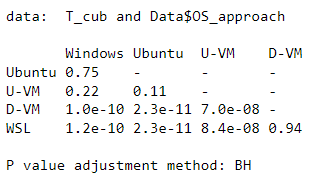
\includegraphics[scale=0.7]{figures/ttest1.PNG}
    \caption{Pairwise t-test as a function of OS approach for transformed data.}
    \label{fig_ttest_1}
\end{figure}


As seen in Figs. \ref{fig_mean_2}. \ref{fig_mean_3}, and \ref{fig_mean_4}, the graph of means and whiskers of time depending on the OS approach and other factors, intuitively it can be seen that Ubuntu is the best for any scenario, followed by Windows, however, it is still not possible to conclude with certainty and say that Ubuntu is better than the others and different from Windows, since statistical analysis is needed for it, that is, post-hoc tests, in this case with the pairwise t-test.

\begin{figure}[tb]
    \centering
    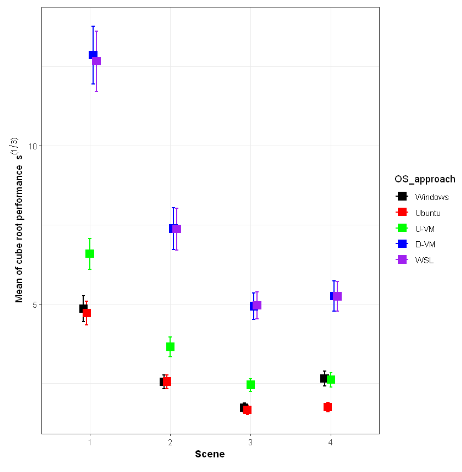
\includegraphics[scale=0.5]{figures/mean2.PNG}
    \caption{Time-transformed mean-whisker plot as a function of the OS approach and the scene.}
    \label{fig_mean_2}
\end{figure}

\begin{figure}[tb]
    \centering
    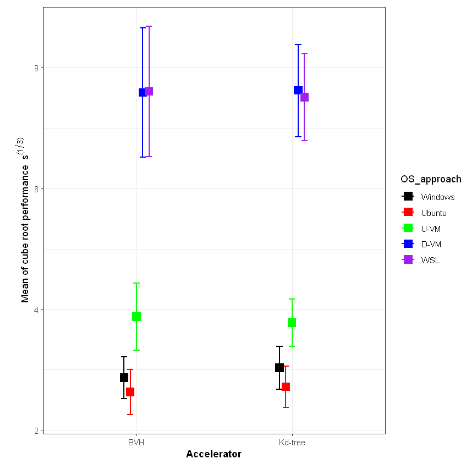
\includegraphics[scale=0.5]{figures/mean3.PNG}
    \caption{Time-transformed mean-whisker plot as a function of the OS approach and the accelerator.}
    \label{fig_mean_3}
\end{figure}

\begin{figure}[tb]
    \centering
    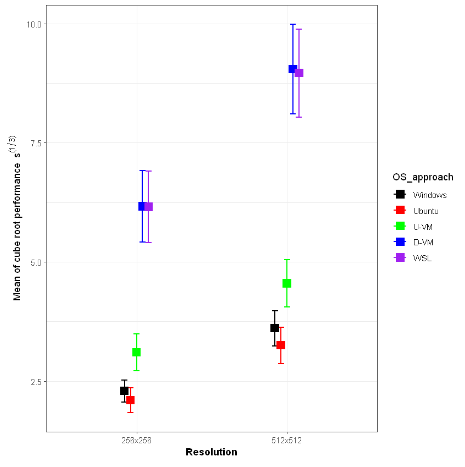
\includegraphics[scale=0.5]{figures/mean4.PNG}
    \caption{Time-transformed mean-whisker plot as a function of the OS approach and the resolution.}
    \label{fig_mean_4}
\end{figure}






\begin{figure}[tb]
    \centering
    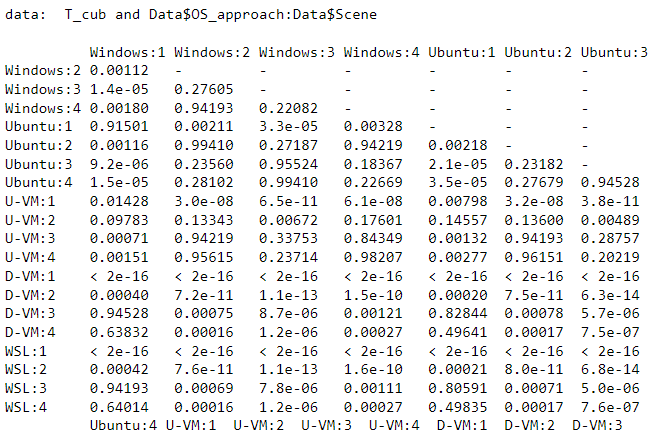
\includegraphics[scale=0.4]{figures/ttest2.PNG}
    \caption{Pairwise t-test as a function of OS approach and the scene for transformed data.}
    \label{fig_ttest_2}
\end{figure}




\begin{figure}[tb]
    \centering
    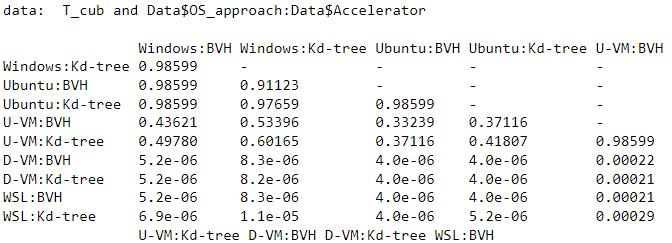
\includegraphics[scale=0.5]{figures/ttest3.PNG}
    \caption{Pairwise t-test as a function of OS approach and the accelerator for transformed data.}
    \label{fig_ttest_3}
\end{figure}




\begin{figure}[tb]
    \centering
    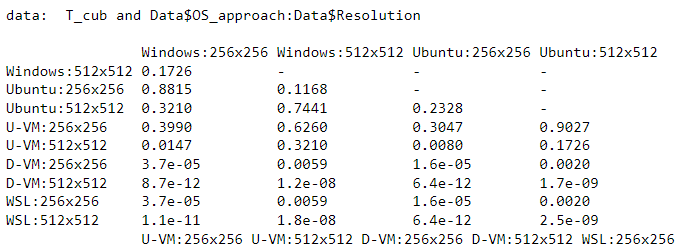
\includegraphics[scale=0.5]{figures/ttest4.PNG}
    \caption{Pairwise t-test as a function of OS approach and the resolution for transformed data.}
    \label{fig_ttest_4}
\end{figure}

Figs. \ref{fig_ttest_2}. \ref{fig_ttest_3}, and \ref{fig_ttest_4} present the tables of the pairwise t-test of the Os approach as the main factor in combination with the other factors one by one for the response variable of the transformed time, these tables are cut since they do not present combinations of interest, that is, only those that have to do with the OS approach factor, under equal conditions, and as can be seen, these comparisons of interest are statistically similar, there is no difference between Ubuntu and Windows and Ubuntu with virtual machine, but at least these three do differ from WSL and debian in virtual machine, which in turn are similar.\par



\section{Conclusions and Further Work}
It cannot be said that Ubuntu is better than Windows and Ubuntu in a virtual machine since the three are statistically similar for any scenario, although the whiskers graphs show the tendency for Ubuntu to be faster, followed by Windows and Ubuntu in a virtual machine. .
Yes, it can be said with certainty that for any scenario, Ubuntu, Windows and Ubuntu in a virtual machine are better and statistically different than Debian in a virtual machine and WSL, which in turn, these two are statistically similar, so there is no major difference between Debian.\par
As future work, this work can be improved by collecting more repetitions of the data, to send it to the ANDESCON conference. Papers Submission is in June 12th, 2022. Under the topic Computer and Software Engineering.

\bibliographystyle{IEEEtran}
\bibliography{bibliography.bib}
%https://www.quora.com/How-can-I-test-data-for-a-uniform-distribution
%http://rstudio-pubs-static.s3.amazonaws.com/433558_30d5068dd9fe45d58243c018c7582fc0.html
%https://stackoverflow.com/questions/44912747/plot-histogram-for-discrete-data

\end{document}

